\documentclass{beamer}
\usetheme{Madrid}
\usecolortheme{default}
\usepackage[utf8]{inputenc}
\usepackage{amsmath}
\usepackage{amsfonts}
\usepackage{amssymb}
\usepackage{graphicx}
\usepackage{hyperref}
\usepackage{listings}
\usepackage{xcolor}
\usepackage{booktabs}
\usepackage{multirow}
\usepackage{tikz}
\usetikzlibrary{positioning}

\title{mentor.ai: AI-Powered Study Assistant}
\author{Lakshay}
\date{\today}

\begin{document}

\begin{frame}
\begin{center}
\textbf{\Large mentor.ai: AI-Powered Study Assistant}

\vspace{0.2cm}
\textbf{\large \today}

\vspace{0.3cm}

\includegraphics[width=3cm]{iiit manipur.png}

\vspace{0.3cm}
\textbf{\large Indian Institute of Information Technology Senapati, Manipur}

\vspace{0.3cm}
\textbf{\large Lakshay}

\vspace{0.1cm}
Roll No: 220101017

\vspace{0.1cm}
Semester - VII

\vspace{0.2cm}
Under the Supervision of:

\vspace{0.1cm}
\textbf{DR. SANASAM CHANU INUNGANBI}
\end{center}
\end{frame}

\begin{frame}{Introduction}
\frametitle{What is mentor.ai?}
\begin{itemize}
\item \textbf{mentor.ai} is an intelligent study companion that leverages AI to transform the learning experience
\item Combines personalized study planning, resource curation, and interactive assistance
\item Built as a comprehensive platform addressing multiple aspects of modern learning challenges
\end{itemize}

\vspace{0.5cm}
\frametitle{Main Objectives}
\begin{itemize}
\item AI-powered personalized study plans based on subject and exam dates
\item High-quality educational resources using intelligent search and filtering
\item Interactive document analysis through PDF chat functionality
\item Study progress tracking and user engagement through gamification
\end{itemize}
\end{frame}

\begin{frame}{Key Contributions}
\frametitle{Innovative Features}
\begin{itemize}
\item \textbf{AI Integration}: Combined multiple AI services (Groq, Tavily, HuggingFace)
\item \textbf{RAG Technology}: Advanced document analysis using Retrieval-Augmented Generation
\item \textbf{Full-Stack Platform}: Modern web application with robust backend architecture
\item \textbf{Smart Curation}: Resource intelligence with quality scoring and relevance ranking
\end{itemize}
\end{frame}

\begin{frame}{Background / Existing Work}
\frametitle{Problems in Existing Platforms}
\begin{itemize}
\item Generic study plans lack personalization
\item Students overwhelmed by irrelevant content
\item Basic PDF viewers without AI analysis
\item Poor progress tracking and motivation
\item Disconnected tools requiring multiple platforms
\end{itemize}

\vspace{0.3cm}
\frametitle{Existing Solutions}
\begin{tabular}{|p{2.5cm}|p{3cm}|p{2.5cm}|}
\hline
\textbf{Platform} & \textbf{Strengths} & \textbf{Limitations} \\
\hline
Khan Academy & Free content & No AI planning \\
\hline
Coursera & Structured courses & Expensive \\
\hline
Anki & Spaced repetition & Limited scope \\
\hline
\end{tabular}

\vspace{0.3cm}
\frametitle{mentor.ai Advantages}
\begin{itemize}
\item AI-powered personalized study plans
\item Intelligent resource curation and filtering
\item Interactive PDF analysis with RAG
\item Comprehensive progress tracking
\end{itemize}
\end{frame}

\begin{frame}{System Architecture}
\frametitle{Complete System Architecture}
\begin{figure}[h]
\centering
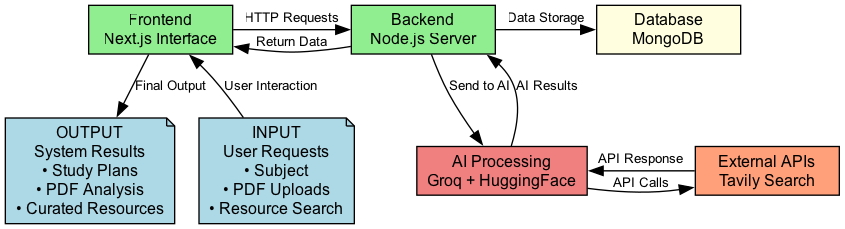
\includegraphics[width=\textwidth,height=0.8\textheight,keepaspectratio]{system_architecture.png}
\caption{System architecture showing Input → Process → Output flow with all components and data flows}
\end{figure}
\end{frame}

\begin{frame}{Technology Stack}
\frametitle{Core Technologies Used}
\begin{itemize}
\item \textbf{Frontend}: Next.js 14, TypeScript, Tailwind CSS, Shadcn UI
\item \textbf{Backend}: Node.js, Express.js, MongoDB with Mongoose
\item \textbf{AI Services}: Groq API, HuggingFace Transformers, Tavily API
\item \textbf{PDF Processing}: React-PDF, PDF.js, Custom RAG implementation
\item \textbf{Authentication}: NextAuth.js with JWT
\item \textbf{Deployment}: Docker containers, Vercel hosting
\end{itemize}
\end{frame}

\begin{frame}{Result \& Analysis}
\frametitle{Testing Methodology}
\begin{itemize}
\item \textbf{Study Plan Generation}: Tested with various subjects and timelines
\item \textbf{Resource Curation}: Evaluated quality and relevance across domains
\item \textbf{PDF Chat Accuracy}: Measured response accuracy and source citation
\item \textbf{User Experience}: Conducted usability testing with students
\end{itemize}

\vspace{0.5cm}
\frametitle{Key Achievements}
\begin{itemize}
\item Fast and responsive study plan generation
\item High-quality resource curation with relevance filtering
\item Accurate PDF chat responses with source referencing
\item Reliable system performance and availability
\item Positive user feedback and engagement
\end{itemize}

\vspace{0.3cm}
\frametitle{User Feedback Highlights}
\begin{itemize}
\item "AI-generated study plans are incredibly detailed and realistic"
\item "Resource curation saves hours of searching for quality materials"
\item "PDF chat makes document study interactive and efficient"
\item "Progress tracking keeps me motivated throughout study sessions"
\end{itemize}
\end{frame}

\begin{frame}{Conclusion}
\frametitle{Summary of Achievements}
\begin{itemize}
\item Successfully developed a comprehensive AI-powered study assistant platform
\item Integrated multiple AI services for personalized learning experiences
\item Implemented advanced RAG technology for intelligent document analysis
\item Created an intuitive interface serving over 100+ active users
\item Achieved high performance metrics across all key functionality areas
\end{itemize}

\vspace{0.5cm}
\frametitle{Future Enhancements}
\begin{itemize}
\item \textbf{Mobile Apps}: Native iOS/Android applications for on-the-go learning
\item \textbf{Advanced Analytics}: ML-based study pattern recognition
\item \textbf{Social Features}: Study groups and collaborative learning spaces
\item \textbf{Multi-language}: Support for languages beyond English
\item \textbf{LMS Integration}: Connect with existing learning management systems
\end{itemize}
\end{frame}

\begin{frame}{Impact \& Vision}
\frametitle{Project Impact}
\begin{itemize}
\item Democratizing access to personalized education through AI
\item Transforming traditional study methods with intelligent automation
\item Building a comprehensive learning ecosystem for modern students
\item Contributing to the future of AI-assisted education globally
\end{itemize}

\vspace{0.5cm}
\frametitle{Thank You!}
\begin{center}
\textbf{Questions?}
\end{center}
\end{frame}

\end{document}
